\documentclass[10pt, a4paper]{scrartcl}

\usepackage{vorschule}
\usepackage[
	typ=ab,
	fach=Informatik,
	lerngruppe={Q2-GK},
	nummer=II.2,
	module={Symbole,Lizenzen},
	seitenzahlen=keine,
	farbig,
	lizenz=cc-by-nc-sa-4,
]{schule}

\usepackage[
	kuerzel=Ngb,
	reihe={Rechnernetze},
	version={2020-11-03},
]{ngbschule}

\author{J. Neugebauer}
\title{Fehlerkorrektur}
\date{\Heute}

\setzeAufgabentemplate{ngbnormal}

\newcommand{\letter}[2][1.5cm]{#2 $\Rightarrow$ \luecke{#1}}

\begin{document}
\ReiheTitel

\begin{multicols}{2}\centering
	\vspace*{2mm}
	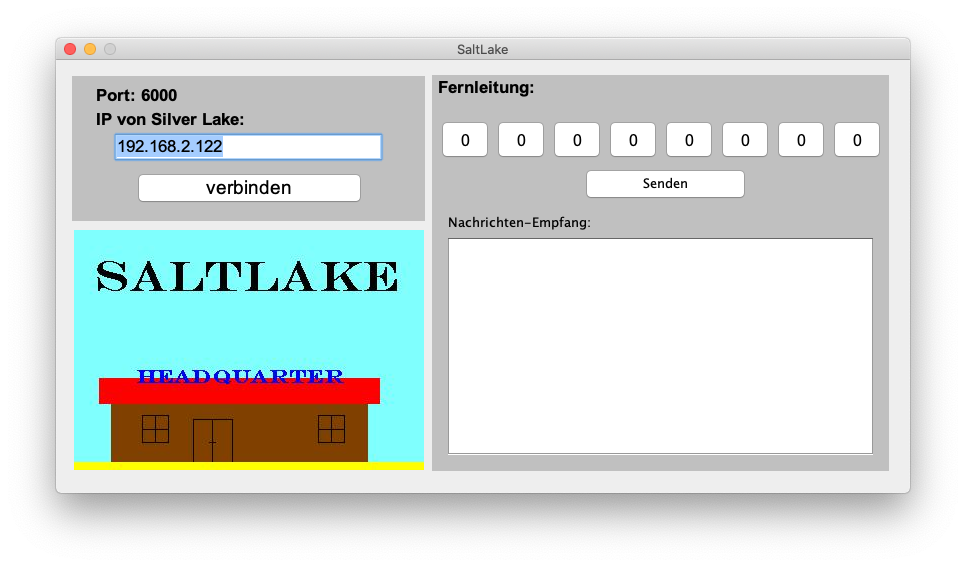
\includegraphics[width=.8\columnwidth]{Q2-GK-AB.II.2-Abb_Saltlake.png}
	
	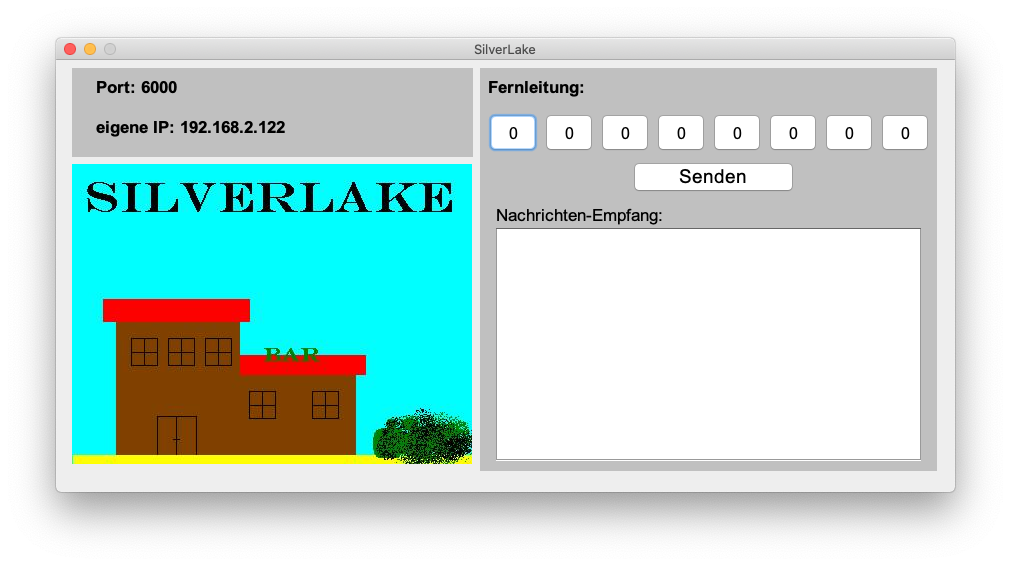
\includegraphics[width=.8\columnwidth]{Q2-GK-AB.II.2-Abb_Silver Lake.png}
\end{multicols}



\end{document}
